\documentclass[border=10pt]{standalone}
% Shared preamble for the VibeStack report diagrams.
% Build one diagram: pdflatex fig_x.tex && pdftoppm -r 220 -png -singlefile fig_x.pdf ../images/fig_x
\usepackage[T1]{fontenc}
\usepackage{lmodern}
\renewcommand{\familydefault}{\sfdefault}
\usepackage{tikz}
\usetikzlibrary{arrows.meta,positioning,shapes.geometric,shapes.misc,fit,backgrounds,calc}
\definecolor{vsred}{RGB}{204,0,0}
\definecolor{lay1}{RGB}{232,240,254}
\definecolor{lay2}{RGB}{230,246,236}
\definecolor{lay3}{RGB}{255,243,224}
\definecolor{lay4}{RGB}{243,232,253}
\tikzset{
  box/.style={draw, rounded corners=3pt, align=center, minimum height=0.95cm, inner sep=5pt, fill=white, font=\small},
  sbox/.style={box, minimum width=2.6cm},
  arrow/.style={-{Stealth[length=2.4mm]}, thick},
  darrow/.style={arrow, dashed},
  lbl/.style={font=\scriptsize, fill=white, inner sep=1.5pt},
  decision/.style={draw, diamond, aspect=2.1, align=center, inner sep=1pt, font=\small, fill=white},
  term/.style={draw, rounded rectangle, minimum width=2.4cm, minimum height=0.9cm, font=\small\bfseries, fill=white},
}

\begin{document}
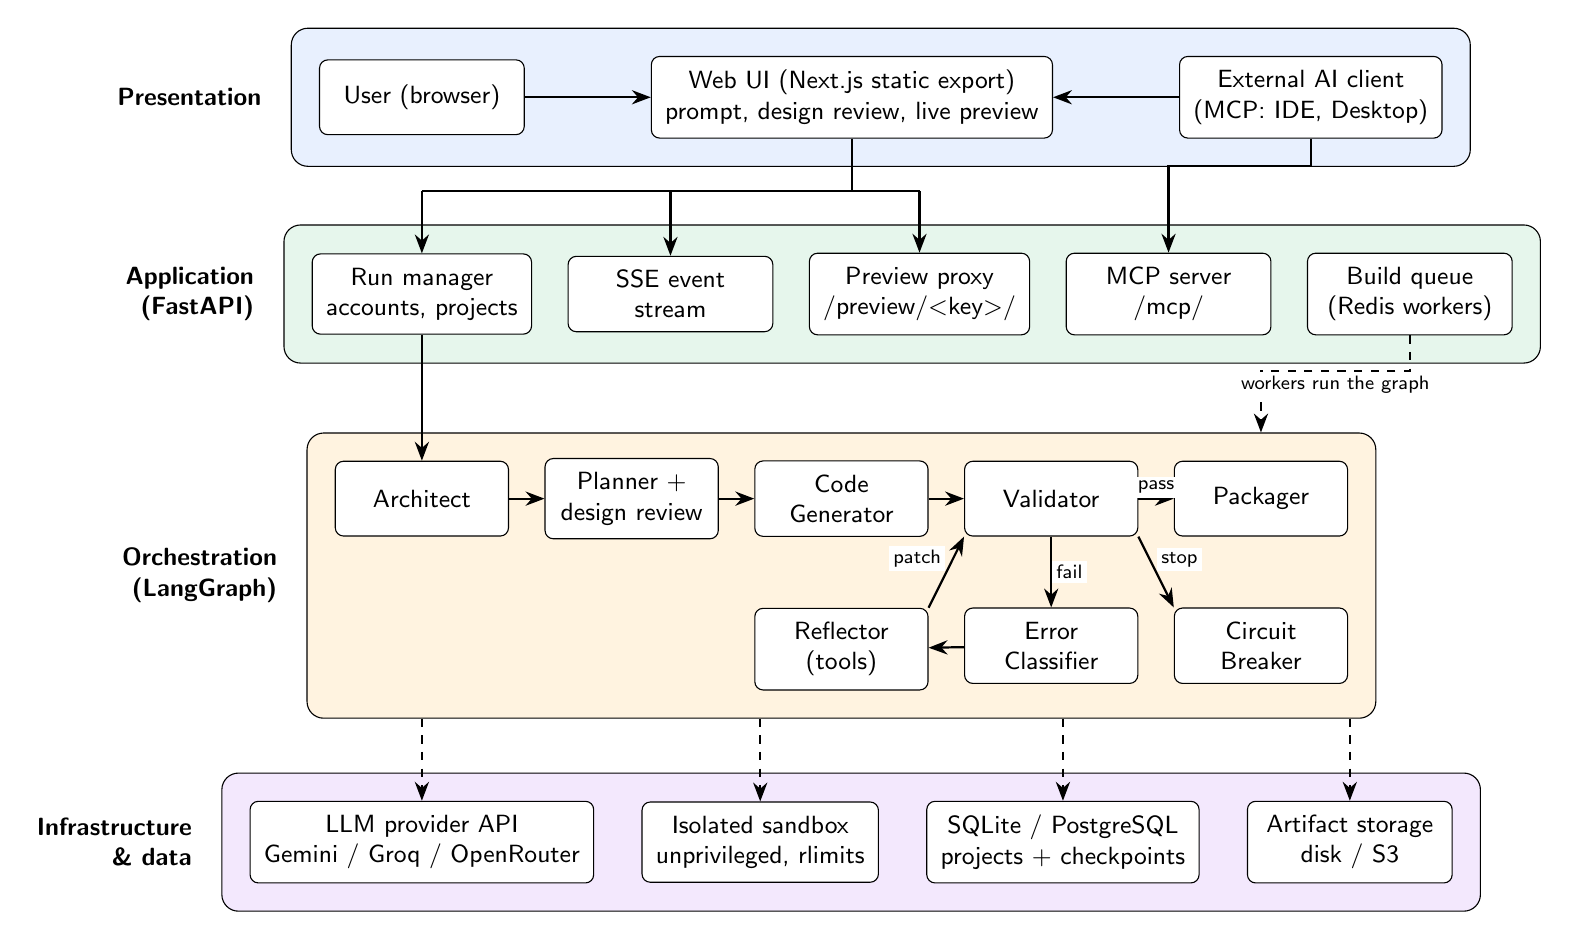
\begin{tikzpicture}[node distance=0.5cm and 0.45cm]
% Presentation
\node[sbox] (user) {User (browser)};
\node[sbox, right=1.6cm of user, minimum width=4.2cm] (ui) {Web UI (Next.js static export)\\ prompt, design review, live preview};
\node[sbox, right=1.6cm of ui] (ide) {External AI client\\(MCP: IDE, Desktop)};
% Application
\node[sbox, below=1.5cm of user] (runs) {Run manager\\accounts, projects};
\node[sbox, right=of runs] (sse) {SSE event\\stream};
\node[sbox, right=of sse] (prev) {Preview proxy\\/preview/\textless key\textgreater/};
\node[sbox, right=of prev] (mcp) {MCP server\\/mcp/};
\node[sbox, right=of mcp] (queue) {Build queue\\(Redis workers)};
% Orchestration
\node[sbox, below=1.6cm of runs, minimum width=2.2cm] (arch) {Architect};
\node[sbox, right=of arch, minimum width=2.2cm] (plan) {Planner +\\design review};
\node[sbox, right=of plan, minimum width=2.2cm] (gen) {Code\\Generator};
\node[sbox, right=of gen, minimum width=2.2cm] (val) {Validator};
\node[sbox, right=of val, minimum width=2.2cm] (pack) {Packager};
\node[sbox, below=0.9cm of gen, minimum width=2.2cm] (refl) {Reflector\\(tools)};
\node[sbox, below=0.9cm of val, minimum width=2.2cm] (cls) {Error\\Classifier};
\node[sbox, below=0.9cm of pack, minimum width=2.2cm] (cb) {Circuit\\Breaker};
% Infrastructure
\node[sbox, below=1.4cm of refl.south -| arch, anchor=north] (llm) {LLM provider API\\Gemini / Groq / OpenRouter};
\node[sbox, right=0.6cm of llm] (sbx) {Isolated sandbox\\unprivileged, rlimits};
\node[sbox, right=0.6cm of sbx] (db) {SQLite / PostgreSQL\\projects + checkpoints};
\node[sbox, right=0.6cm of db] (art) {Artifact storage\\disk / S3};
% Layers
\begin{scope}[on background layer]
\node[draw, rounded corners=6pt, fill=lay1, fit=(user)(ui)(ide), inner sep=10pt] (L1) {};
\node[draw, rounded corners=6pt, fill=lay2, fit=(runs)(queue), inner sep=10pt] (L2) {};
\node[draw, rounded corners=6pt, fill=lay3, fit=(arch)(pack)(cb)(refl), inner sep=10pt] (L3) {};
\node[draw, rounded corners=6pt, fill=lay4, fit=(llm)(art), inner sep=10pt] (L4) {};
\end{scope}
\foreach \L/\t in {L1/Presentation, L2/{Application\\(FastAPI)}, L3/{Orchestration\\(LangGraph)}, L4/{Infrastructure\\\& data}}
  \node[font=\small\bfseries, align=right, anchor=east] at ($(\L.west)+(-0.25,0)$) {\t};
% Edges
\draw[arrow] (user) -- (ui);
\draw[arrow] (ide) -- (ui.east) ;
\coordinate (bus) at ($(ui.south)!0.45!(ui.south |- sse.north)$);
\draw[thick] (ui.south) -- (ui.south |- bus);
\draw[thick] (runs.north |- bus) -- (prev.north |- bus);
\foreach \n in {runs, sse, prev} \draw[arrow] (\n.north |- bus) -- (\n.north);
\draw[arrow] (ide.south) -- ++(0,-0.35) -| (mcp.north);
\draw[darrow] (queue.south) -- ++(0,-0.45) -| node[lbl, pos=0.25, below]{workers run the graph} (pack.north |- L3.north);
\draw[arrow] (runs.south) -- (arch.north);
\draw[arrow] (arch) -- (plan);
\draw[arrow] (plan) -- (gen);
\draw[arrow] (gen) -- (val);
\draw[arrow] (val) -- node[lbl, above]{pass} (pack);
\draw[arrow] (val) -- node[lbl, right]{fail} (cls);
\draw[arrow] (cls) -- (refl);
\draw[arrow] (refl.north east) -- node[lbl, above left]{patch} (val.south west);
\draw[arrow] (val.south east) -- node[lbl, above right]{stop} (cb.north west);
\draw[darrow] (L3.south -| llm) -- (llm.north);
\draw[darrow] (L3.south -| sbx) -- (sbx.north);
\draw[darrow] (L3.south -| db) -- (db.north);
\draw[darrow] (L3.south -| art) -- (art.north);
\end{tikzpicture}
\end{document}
